\section{Calibration} \label{sec:calib}

In this section the various calibration procedures taken in order to minimize the time resolution and enhance both the particle identification (PID) and time of flight (TOF) capabilities of the Start Counter are discussed.

\subsection{Time-Walk Correction} \label{sec:calib_tw}

The time-walk effect is a well understood consequence of leading edge discriminators (LED).  Analog signals of varying amplitudes crossing a fixed threshold, as determined by the discriminator threshold setting, will do so at varying times as illustrated in Fig.~\ref{fig:time_walk_effect}.
	\begin{figure}[!htb]
		\centering
		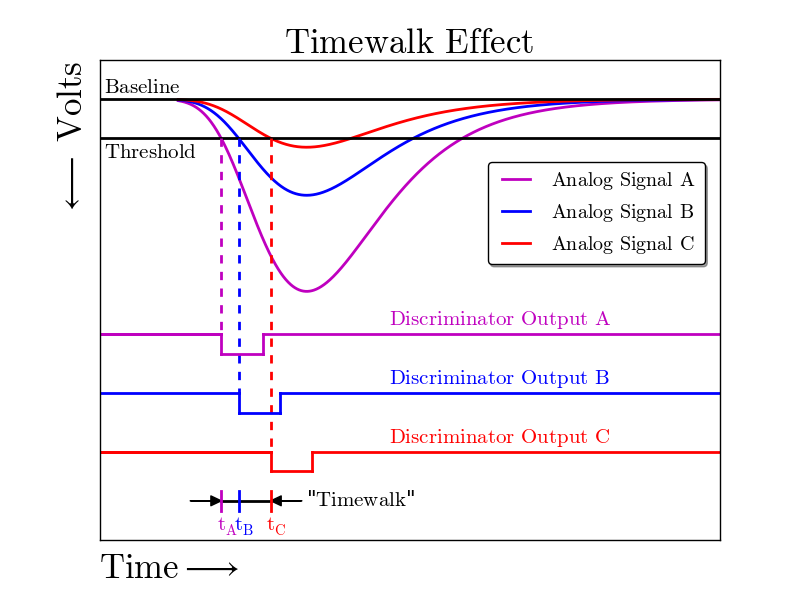
\includegraphics[width=1.0\columnwidth]{calibration/figs/time_walk_effect}
		\caption{Example of the time-walk effect. Three coincident analog signals A, B, \& C of varying amplitudes crossing a fixed threshold in a LED. The discriminator logic output signals vary in time relative to the amplitude of the incoming analog signal.  The signals shown above are simulated analog signals being fed into the LED's thus, they have negative polarity.}
		\label{fig:time_walk_effect}
	\end{figure}
Thus, the corresponding logic signal output from the LED will ``\textit{walk about}'' in time, resulting in an undesirable smearing of the measured ST TDC times.

The FADC250's provide a high resolution pulse time (62.5~ps) that is time-walk independent \cite{pooser16} \cite{dong_fadc}.  Therefore, for events in which both the FADC and TDC register hits in the same channel, the pulse time can serve as a reference time for that event.  The TDC/FADC time difference is given by Eq.~\ref{eq:tdc_adc_tdiff}.
	\begin{equation} \label{eq:tdc_adc_tdiff}
		\delta t_{i} = t^{TDC}_{i} - t^{FADC}_{i}
	\end{equation}
Figure \ref{fig:twdistuncorrch15} shows a typical time-walk spectrum, \textit{i.e.} $\delta t_{i}$ versus the pulse amplitude, for one sector of the ST.
	\begin{figure}[!htb]
		\centering
		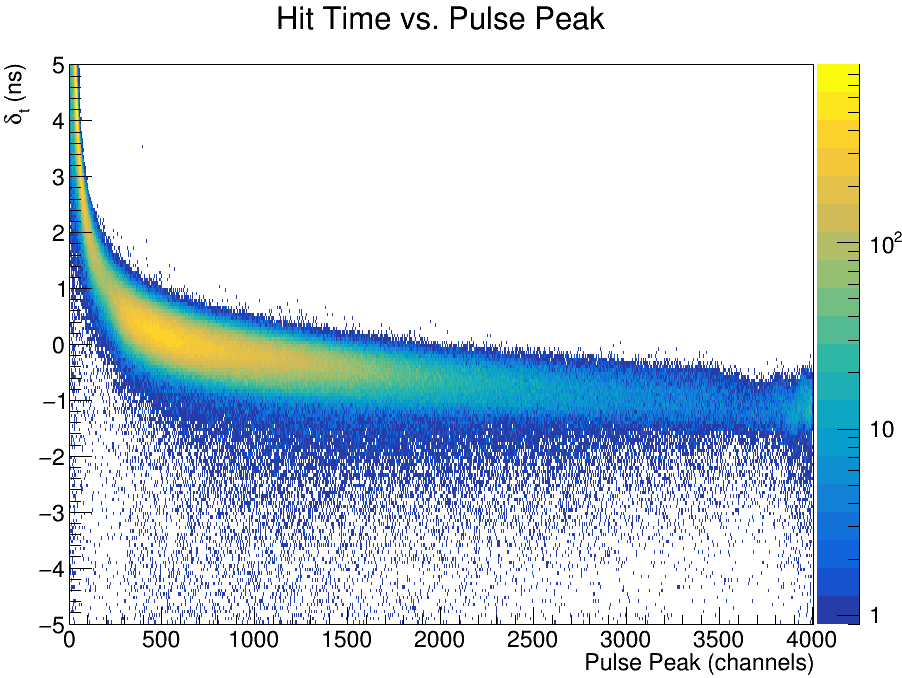
\includegraphics[width=1.0\columnwidth]{calibration/figs/tw_dist_uncorr_ch15}
		\caption{Typical Start Counter time-walk spectrum.  Shown is the time-walk spectrum for sector 15 of the Start Counter during the Spring 2017 run. On the y-axis is $\delta t_{15}$ and on the x-axis is the corresponding pedestal subtracted pulse peak spectrum. From this histogram it is clear that there is a correlation between the amplitude of the analog signal and the time in which the signal crosses the discriminator threshold.}
		\label{fig:twdistuncorrch15}
	\end{figure}
The FADC250's return both the amplitude and integral of events which are above threshold \cite{dong_fadc}.  Since the amplitude better characterizes the ADC pulse profile as compared to the pulse integral, it was utilized for the time-walk corrections.

The non time-walk corrected spectrum illustrates the poor time resolution due to the large spread in time differences occurring among signals close to threshold and the more probable amplitudes being registered in the FADC. From Fig.~\ref{fig:twdistuncorrch15} it is immediately obvious that there exists a correlation between the time and the pulse peak for hits in the ST.  This correlation is nonlinear and requires a polynomial functional form to describe the correlation. Equation~\ref{eq:tw_corr_func_form} from reference \cite{esmith_bcal} was chosen to characterize the correlation between $\delta t_{i}$ and the amplitude of the signal. 
	\begin{equation} \label{eq:tw_corr_func_form}
		f^{w}_{i}\left(a/a^{thresh}_{i}\right) = c0_{i} + \frac{c1_{i}}{(a/a^{thresh}_{i})^{c2_{i}}}
	\end{equation}
In Eq.~\ref{eq:tw_corr_func_form} $f^{w}_{i}$ is the functional form of time-walk fit for the $i^{th}$ sector, while $a$ and $a^{thresh}_{i}$ are the pulse peak and discriminator threshold converted to ADC units respectively.  Furthermore, $c0_{i}, c1_{i}, c2_{i}$ are the time-walk correction fit parameters.

The data in Fig.~\ref{fig:twdistuncorrch15} were fit using Eq.~\ref{eq:tw_corr_func_form} and ROOT's MINUIT $\chi^{2}$ minimization fitting library for pulse peak values ranging from [50, 2100].  An identical fit was carried out for each of the ST sectors.

The most probable value (MPV) of the minimum ionizing peak was chosen to be the location in which the time-walk correction was zero.  This location effectively serves as a reference point for the correction.  As seen in Fig. \ref{fig:pulsepeakch15} a ``pseudo'' MPV was utilized.
	\begin{figure}[!htb]
		\centering
		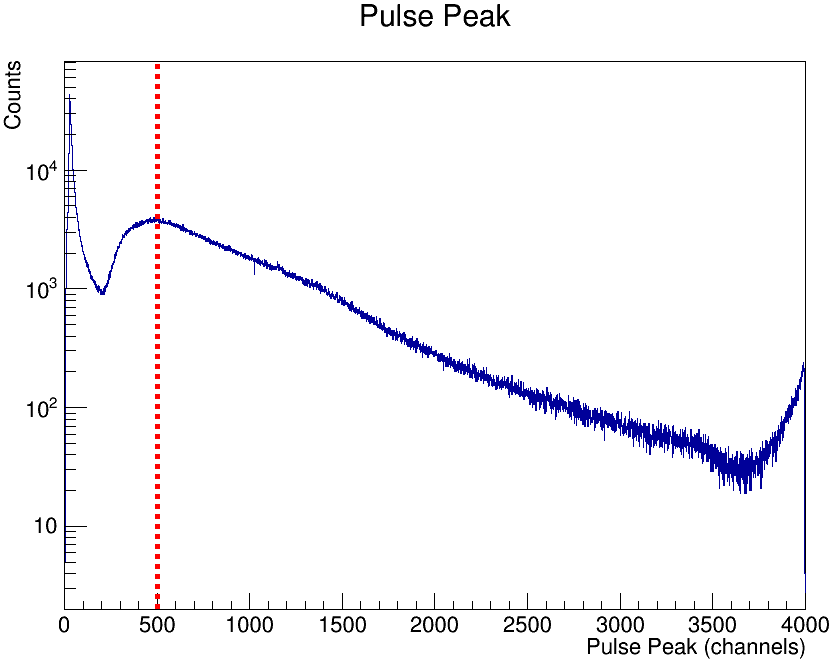
\includegraphics[width=1.0\columnwidth]{calibration/figs/pulse_peak_ch15}
		\caption{Typical pulse peak minimum ionizing distribution.  Shown is the pulse peak minimum ionizing distribution for sector 3 during the Spring 2017 run. The red, vertical, dashed line in the histogram corresponds to the ``pseudo'' MPV ($a^{0}_{15}$) which was determined to be 500.}
		\label{fig:pulsepeakch15}
	\end{figure}
The ``pseudo'' MPV $(a^{0}_{i})$ was determined on a sector by sector basis by simply acquiring the pulse peak channel which had the most number of entries after the pulse peak channel 200.  The large spike in the pulse peak spectrum at very low pulse peak values are due to electromagnetic background events clipping threshold and do not correspond to a true minimum ionizing particle traversing the scintillator medium.

With all the necessary parameters, \textit{i.e.} $a^{0}_{i},\ c0_{i},\ c1_{i},\ c2_{i}$, determined the time-walk correction factor can be applied to the original TDC time.  The functional form of the time-walk corrected time is given by Eq. \ref{eq:tw_corr}.
	\begin{equation} \label{eq:tw_corr}
		T^{w}_{i} = t^{TDC}_{i} - f^{w}_{i}(a/a^{thresh}_{i}) + f^{w}_{i}(a^{0}_{i}/a^{thresh}_{i})
	\end{equation}
Once the time walk corrections have been applied, the corrected timing distributions appear much more uniform in nature and exhibit a factor 1.75 improvement in resolution \cite{pooser16}.  Figure~\ref{fig:twdistcorrch15} illustrates the vast improvement in the time difference spectrum ($\delta t_{15}$) due to the applied time-walk corrections.
	\begin{figure}[!htb]
		\centering
		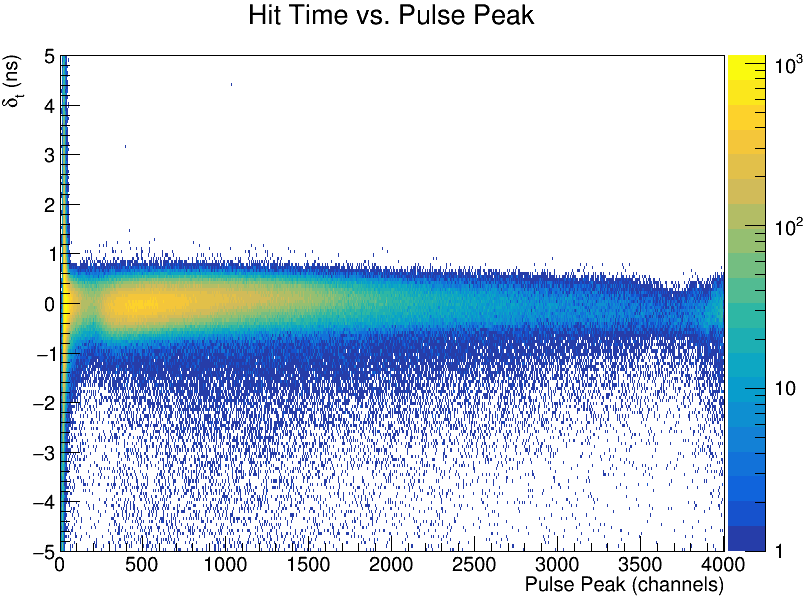
\includegraphics[width=1.0\columnwidth]{calibration/figs/tw_dist_corr_ch15}
		\caption{Time-walk corrected time difference spectrum.  Shown is the time-walk corrected time difference spectrum for sector 3 during the Spring 2017 run. The time-walk corrected time difference spectrum has $\sigma_{\delta t_{15}} \approx 270 ps$}
		\label{fig:twdistcorrch15}
	\end{figure}
In Fig.~\ref{fig:sttimeoverlaych15} illustrates the $\delta t_{15}$ distribution and the relative effects of the aforementioned time-walk correction.
	\begin{figure}[!htb]
		\centering
		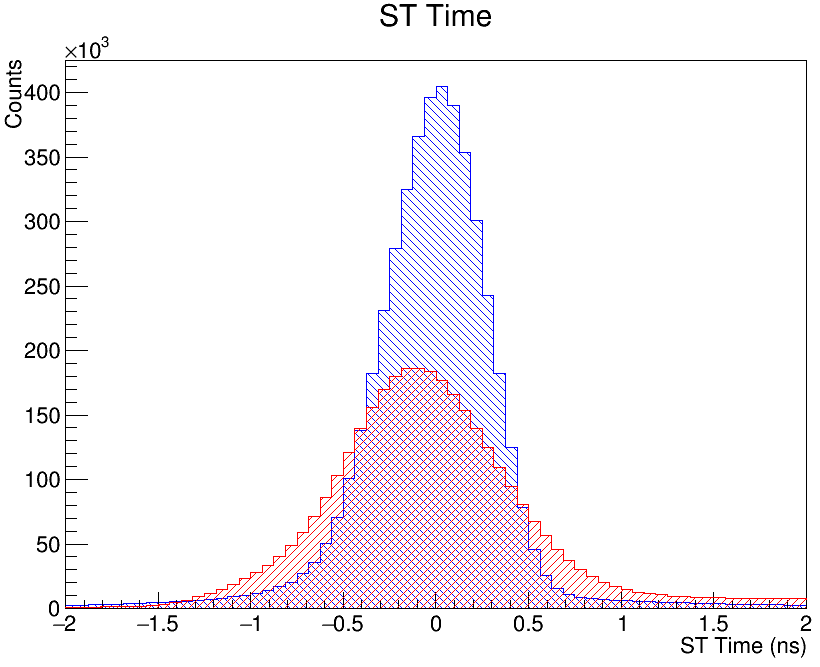
\includegraphics[width=1.0\columnwidth]{calibration/figs/st_time_overlay_ch15}
		\caption{Comparison of pre and post self-timing distributions.}
		\label{fig:sttimeoverlaych15}
	\end{figure}
